% Copyright (c) 2026 Morwenn
% SPDX-License-Identifier: MIT

\documentclass{standalone}
\usepackage{bm, pgf, tikz}
\usetikzlibrary{arrows, automata, backgrounds, positioning}

\begin{document}
    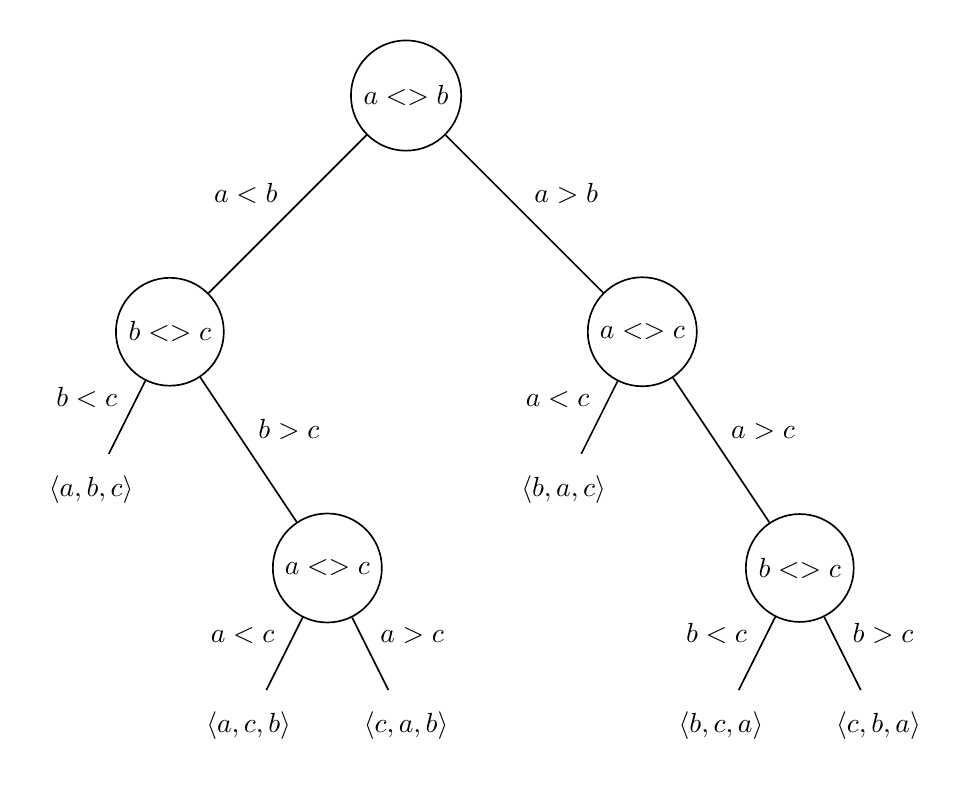
\begin{tikzpicture}[
            background rectangle/.style={fill=white},
            show background rectangle,
            auto,
            on grid,
            node distance = 1.3cm and 3cm,
            semithick
        ]

        \tikzstyle{every state}=[
            %draw=none,
            shape=circle,
            fill=white
        ]
        
        \node[state] (n0) at (5,9) {$a<>b$};
        \node[state] (n1) at (2,6) {$b<>c$};
        \node[state] (n2) at (8,6) {$a<>c$};
        \node[state] (n3) at (4,3) {$a<>c$};
        \node[state] (n4) at (10,3) {$b<>c$};

        \tikzstyle{every state}=[
            draw=none,
            shape=rectangle,
            fill=white
        ]
        
        \node[state] (abc) at (1,4) {$\langle a, b, c \rangle$};
        \node[state] (acb) at (3,1) {$\langle a, c, b \rangle$};
        \node[state] (bac) at (7,4) {$\langle b, a, c \rangle$};
        \node[state] (bca) at (9,1) {$\langle b, c, a \rangle$};
        \node[state] (cab) at (5,1) {$\langle c, a, b \rangle$};
        \node[state] (cba) at (11,1) {$\langle c, b, a \rangle$};

        \path[-] (n1) edge node {$a < b$} (n0);
        \path[-] (n0) edge node {$a > b$} (n2);
        \path[-] (abc) edge node {$b < c$} (n1);
        \path[-] (n1) edge node {$b > c$} (n3);
        \path[-] (bac) edge node {$a < c$} (n2);
        \path[-] (n2) edge node {$a > c$} (n4);
        \path[-] (acb) edge node {$a < c$} (n3);
        \path[-] (n3) edge node {$a > c$} (cab);
        \path[-] (bca) edge node {$b < c$} (n4);
        \path[-] (n4) edge node {$b > c$} (cba);

    \end{tikzpicture}
\end{document}
